\documentclass{article}
\pagestyle{empty}
\usepackage{tikz}
\usetikzlibrary{arrows.meta,decorations.pathreplacing}
\definecolor{diagOrange}{RGB}{240,105,26}
\definecolor{boxFill}{RGB}{239,239,239}
\definecolor{boxStroke}{RGB}{154,154,154}
\definecolor{inkGray}{RGB}{51,51,51}
\begin{document}
\noindent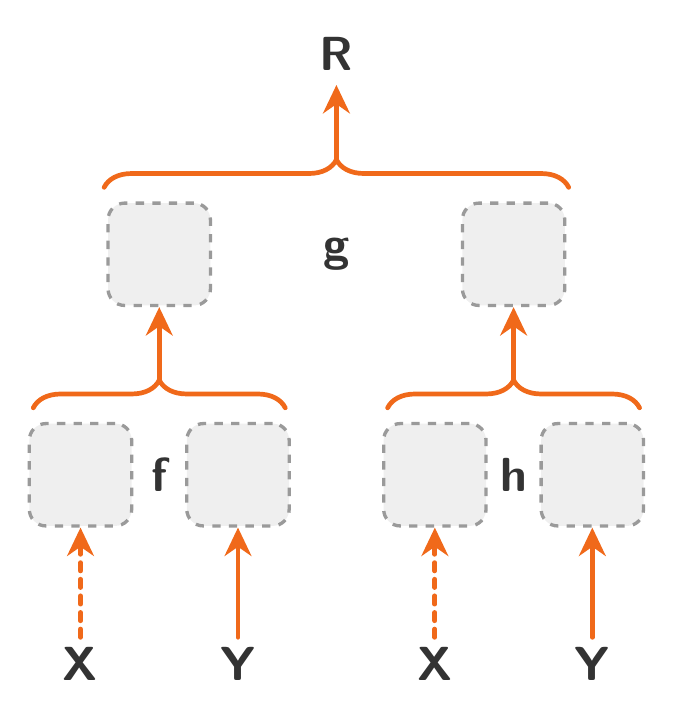
\begin{tikzpicture}[
  >={Stealth[length=3.6mm,width=3.4mm]},
  line join=round,
  slot/.style={draw=boxStroke, dashed, line width=1.2pt, rounded corners=6pt,
               fill=boxFill, minimum size=1.3cm},
  flow/.style={diagOrange, line width=1.7pt, line cap=round, ->},
  flowdash/.style={diagOrange, line width=1.7pt, line cap=round, dashed, ->},
  brace/.style={diagOrange, line width=1.7pt, line cap=round,
                decorate, decoration={brace, amplitude=10pt}},
  lbl/.style={inkGray, font=\sffamily\bfseries\LARGE},
]
  % leaves: the same X, Y feeding each of f and h
  \node[lbl] (Xf) at (1.0,0.2) {X};
  \node[lbl] (Yf) at (3.0,0.2) {Y};
  \node[lbl] (Xh) at (5.5,0.2) {X};
  \node[lbl] (Yh) at (7.5,0.2) {Y};

  % f and h argument slots
  \node[slot] (fL) at (1.0,2.6) {};
  \node[slot] (fR) at (3.0,2.6) {};
  \node[slot] (hL) at (5.5,2.6) {};
  \node[slot] (hR) at (7.5,2.6) {};

  % f and h braces (labels centred)
  \draw[brace] (0.4,3.45) -- (3.6,3.45);   % f, tip at x=2.0
  \node[lbl] at (2.0,2.6) {f};
  \draw[brace] (4.9,3.45) -- (8.1,3.45);   % h, tip at x=6.5
  \node[lbl] at (6.5,2.6) {h};

  % g's two argument slots + brace
  \node[slot] (gL) at (2.0,5.4) {};
  \node[slot] (gR) at (6.5,5.4) {};
  \draw[brace] (1.3,6.25) -- (7.2,6.25);   % g, tip at x=4.25
  \node[lbl] at (4.25,5.4) {g};

  % wiring (add "mirror" to a brace decoration if its tip points down)
  \draw[flowdash] (Xf) -- (fL);            % X
  \draw[flow]     (Yf) -- (fR);            % Y
  \draw[flowdash] (Xh) -- (hL);            % X
  \draw[flow]     (Yh) -- (hR);            % Y
  \draw[flow] (2.0,3.78) -- (gL);          % f -> g's left slot
  \draw[flow] (6.5,3.78) -- (gR);          % h -> g's right slot
  \draw[flow] (4.25,6.58) -- (4.25,7.55);  % g -> R
  \node[lbl] (R) at (4.25,7.95) {R};
\end{tikzpicture}
\end{document}
